\documentclass[10pt,a4paper]{article}
\usepackage[utf8]{inputenc}
\usepackage[parfill]{parskip}
\usepackage[section]{placeins}
\usepackage{subfig}
\usepackage{graphicx}
\usepackage{array}
\usepackage{tabularx}
\usepackage[scientific-notation=true]{siunitx}
\usepackage{amsmath}
\usepackage{hyperref}
\usepackage{epigraph}
\author{Dominik Nerger (i6146759)}
\title{Text Mining South Park}
\date{\today}

\begin{document}
	\maketitle
	
	\tableofcontents
	\newpage
	\clearpage
	\setcounter{page}{1}
	\section{Introduction}
	\epigraph{ And tell everyone in the past for us, that no one single answer... is ever the answer. }{UAA Leader, Ep. Go God Go XII}

	South Park is an animated series revolving around the four boys Stan Marsh, Kyle Broflovski, Eric Cartman and Kenny McCormick who live in South Park, Colorado. South Park has the third most episodes in regard to American animated TV series, totaling 277 episodes over 20 seasons. 
	
	Because of the huge amount of episodes, it is an interesting target for the practical assignment, which is part of the course \textit{Information Retrieval \& Text Mining}, with the possibility of acquiring new insights into a TV series that is used to satirize American culture. 

	
	At first, all libraries that were used will be presented. Afterwards, the data set and the used corpora are introduced.  Then the pre-processing tasks that are performed on the data set will be explained. Next, the results and visualization will be discussed while explaining why and how everything has been implemented.
	
	
	As part of the assignment is to answer combinations of W-questions, this report will also focus on the two combinations that were implemented, namely the \textit{why-when} in the form of a sentiment timeline and the \textit{what-when} in form of a topic timeline.
	In the end, a conclusion will be drawn and possible improvements for the future will be discussed.	
	
	
	The repository is available on GitHub\footnote{\url{https://github.com/dnerger/South-Park-Text-Mining}}.
	\section{Libraries}
	
	All scripts have been programmed in \textit{R}. To execute the scripts, R needs to be installed. To view temporary files that are executed during runtime, e.g. the corpus or a TermDocumentMatrix, it is advised to install RStudio. The libraries necessary for each script are imported at the top of each script, if they are not installed they can be installed by executing:
	
	\begin{verbatim}
	install.packages("library-name")
	\end{verbatim}
	
	In the following, all libraries that are related to Text Mining techniques will be introduced shortly.
	
	The library \textbf{tm} is the Text Mining package of R, which enables pre-processing of data sets and allows to build the corpus. \textbf{RWeka} is a collection of machine learning algorithms for data mining tasks. \textbf{NMF} introduces the Non-negative Matrix Factorization to R.
	\textbf{NLP} and \textbf{OpenNLP} are libraries that provide Natural Language Processing techniques and are used for NER-Tagging. \textbf{syuzhet} uses tokenized input to extract sentiments and emotions and contains the three sentiment lexicons \textit{bing}, \textit{afinn} and \textit{nrc}.
	The package \textbf{stm} is used for Structural Topic Modeling  which is LDA with additional meta-data and can be visualized using the package \textbf{LDAvis}.
	Libraries used for visualization include \textbf{igraph},\textbf{ggplot2}, \textbf{ggraph}, \textbf{viridis} and \textbf{wordcloud}.
	
	\section{Data set}	
	The data set spans from seasons \textbf{1} to \textbf{18}, adding up to 257 episodes overall with a file size of 5.41MB. It contains 70896 rows, with each row possessing information about the \textbf{season}, \textbf{episode}, \textbf{character} and \textbf{line} and is available as a \textit{.csv} file.
	
	The data set has been crawled by Bob Adams and is available to download on GitHub\footnote{\url{https://github.com/BobAdamsEE/SouthParkData}}. It has been assembled by crawling the South Park Archives\footnote{\url{http://southpark.wikia.com/wiki/South_Park_Archives}}. The code of this GitHub repository is not available to the public.
	
	 I made an attempt at a crawl with the R package \textbf{rvest}, which is able to harvest data from websites.  However, the \textit{html} data of the episode scripts provided on the South Park Archives differ between episodes. For 16 of 20 seasons, the whole episode needs to be pre-processed manually because the \textbf{line} and \textbf{character} are extracted individually and can not be merged because of random whitespace lines that are introduced by \textbf{rvest}.
	 
	 In the scripts, the data set is used in three different variations:
	 \begin{enumerate}
	 \item \textit{dialogue} - each entry holds information about season, episode, character and line
	 \item \textit{by.season} - each entry holds information about season and the complete script for that season
	 \item \textit{by.episode} - each entry holds information about that episode, season and script for that episode
	 \end{enumerate}
	 
	 Both \textit{by.episode} and \textit{by.season} are created by using the data from \textit{dialogue}.
	
	
	
	
	\section{Pre-processing}
	In general, the standard pre-processing tasks are executed on the corpus. Depending on the later use, different packages perform these.
	The package \textbf{tm} is used to convert the corpus to lower case, remove punctuation and numbers as well as strip whitespaces. Furthermore, stopwords are removed using the stopword list from the Snowball stemmer project. The corpus is stemmed using Porter's stemming algorithm.\footnote{\url{http://snowball.tartarus.org/algorithms/english/stop.txt}}
	
	 It is used together with several DocumentTerm- and TermDocument-Matrices. From these DTMs/TDMs, sparse terms are removed. The maximum allowed sparsity depends on the data set and the intended use, with the allowed percentage being higher for the \textit{by.episode} data set in comparison to \textit{by.season} because there are more documents in the \textit{by.episode} data set. 
	
	The pre-processing for the Structural Topic Model is done with the same tasks, however those are performed by the package \textbf{stm} itself.
	
	For the Named Entity Recognition and Sentiment Annotation with package \textbf{openNLP}, no pre-processing tasks are performed. They can be executed and might improve the overall runtime, but it does not change the overall result. Especially stemming and the lower case convertion could decrease the results because stemmed or lower case entities, as well as the sentiments that are mined, will not be recognized.

	
	\newpage
	\section{Results and visualization}
	
	To sufficiently present the results and the corresponding visualization, each relevant script will present them in their own subsection.
	
	\subsection{Wordclouds}
	To start to gain an insight into South Park, I started with building wordclouds that display the most frequent words to see what South Park is about. However, even with stopwords removed, the words that are most frequent mostly include words such as \textit{get, just} and \textit{now}. From these words, nothing about the TV show can be derived. 
	
	To get meaningful answers to what is important in and characteristic for South Park, the corpus is built with a term frequency-inverse document frequency (tf-idf) weight, which reflects how important each term is to the corresponding document in the corpus.
	\begin{figure}[!h]
  \centering
  \begin{minipage}[b]{0.45\textwidth}
    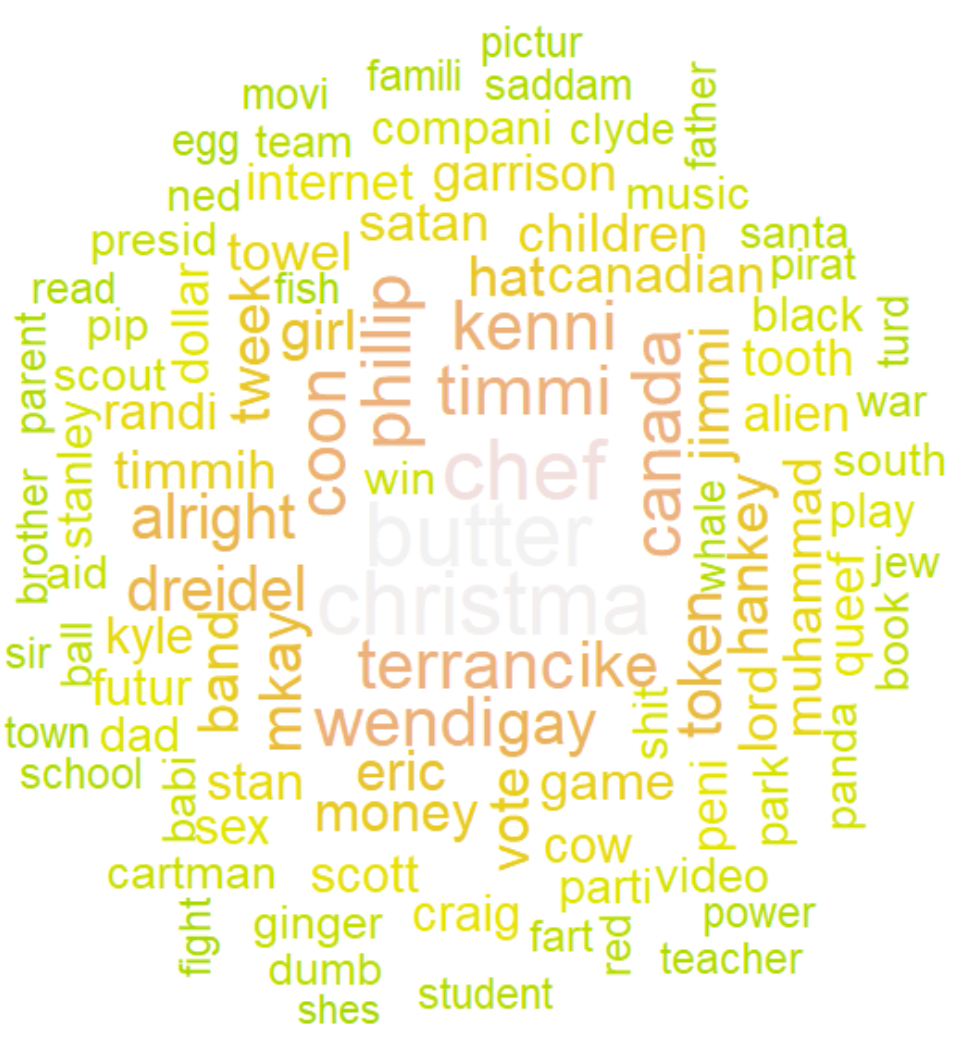
\includegraphics[width=\textwidth]{images/WordCloud-TFIDF-episode.png}
    \caption{ Terms with highest TF-IDF score - \textit{by.episode}}
	\label{fig:WordCloud-TFIDF-ep}
  \end{minipage}
  \hfill
  \begin{minipage}[b]{0.5\textwidth}
    \includegraphics[width=\textwidth]{images/WordCloud-TFIDF.png}
    \caption{Terms with highest TF-IDF score - \textit{by.season}}
	\label{fig:WordCloud-TFIDF-s}
  \end{minipage}
\end{figure}
	
	With this weighting, the terms that are most important over all 18 seasons can be derived, as can be seen in Figures~\ref{fig:WordCloud-TFIDF-ep} and~\ref{fig:WordCloud-TFIDF-s}.
	
		The difference between the wordclouds descends from the different \textit{idf} weights for the data sets \textit{by.season} and \textit{by.episode}. The words in Figure~\ref{fig:WordCloud-TFIDF-ep} show the names of secondary characters such as Butters, Kenny and Wendy. These characters are not featured in Figure~\ref{fig:WordCloud-TFIDF-s} since they do appear in every season, but not in every episode. This leads to their tf-idf weight being zero in the \textit{by.season} data set.
		
			\begin{figure}[h]
	\centering
	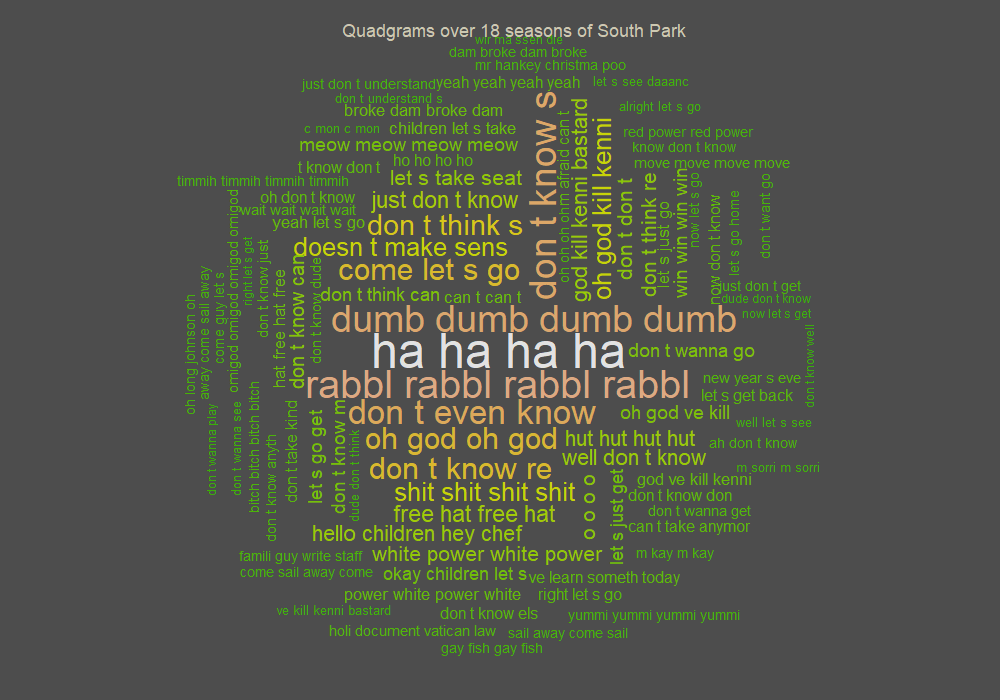
\includegraphics[scale=0.5]{images/WordCloud-ngram.png}
	\caption{Wordcloud containing ngrams (n=4) by frequency}
	\label{fig:WordCloud-ngram}
	\end{figure}
		
		Figure~\ref{fig:WordCloud-ngram} shows the most frequent quadgram phrases without stopwords included. This includes sentences like the trademark phrase "Oh my god, they killed Kenny", which is shown as "oh god kill kenni" because this was calculated with the pre-processed corpus.

	
	
	\subsection{Co-occurences and dendrogram}
	To gain insight into the relations between characters and to confirm the major characters of South Park, which are Stan, Kyle and Cartman, I decided to visualize the 20 characters with the most lines.
	
	As can be seen in Figure~\ref{fig:SpeakingPercentage}, Cartman is the character with most lines overall, with Stan and Kyle, as well as Butters and Randy being other major characters. This has been implemented by aggregating all lines for a character and then calculating the percentages in respect to the overall lines.
	
	\begin{figure}[h]
	\centering
	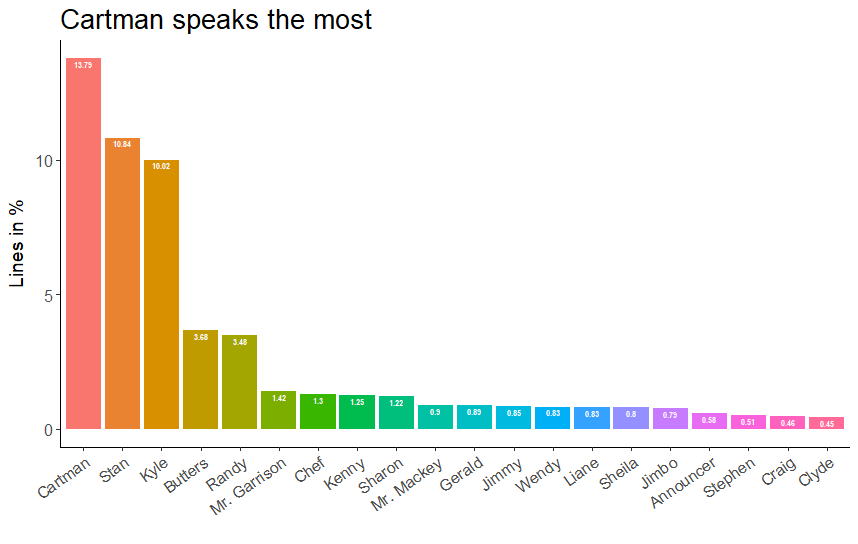
\includegraphics[scale=0.5]{images/speakingPercentage.png}
	\caption{Speaking percentage for 20 major characters}
	\label{fig:SpeakingPercentage}
	\end{figure}	
	
	
	However, this does not show the relations between the characters. To visualize this, I decided to create a co-occurence network by creating a DocumentTermMatrix that contains the characters as terms and the unique episode number as document. The value in each entry is the amount of lines for the character in the specific episode.
	
	 By using the formula $C = A^tA$ with A as the DocumentTermMatrix, I created a TermTermMatrix that contains the co-occurences between lines of characters, resulting in the co-occurences of the 20 most relevant characters in South Park.
	
	
	\begin{figure}[h]
	\centering
	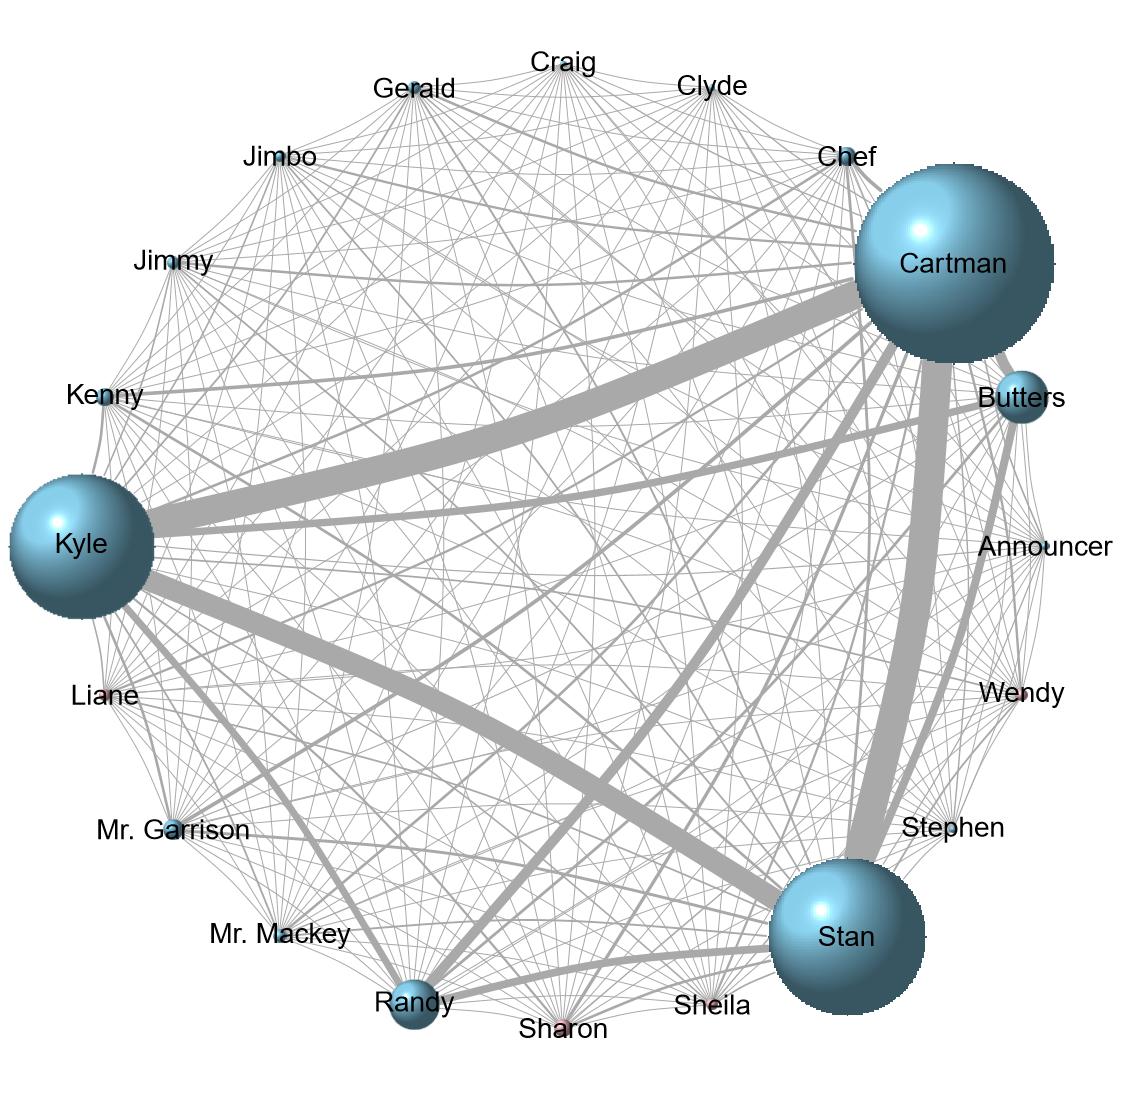
\includegraphics[scale=0.6]{images/CoOccurenceMatrix.png}
	\caption{Co-occurence network}
	\label{fig:CoOccurence}
	\end{figure}		
	
	
	As can be seen in Figure~\ref{fig:CoOccurence}, all 20 major characters interact in some way throughout all 257 episodes, with Cartman, Kyle and Stan being characters that are closely tied together. 
	
	Since it is hard to derive the relations between the characters from Figure~\ref{fig:CoOccurence}, I decided to use a cluster dendrogram to visualize which characters have the most episodes in common. This is accomplished by normalizing the DocumentTermMatrix in regard of the row sums and then applying hierarchical clustering with the Manhattan distance.
	
	Figure~\ref{fig:Dendrogram} shows the dendrogram clustering the characters. The further down the node of two characters splits, the more episodes these characters have in common. This shows once again that the major characters Cartman, Stan and Kyle are closely tied together. Furthermore, interesting connections between the students Clyde and Craig as well as the fathers Stephen and Randy can be derived.
	
		\begin{figure}[h]
	\centering
	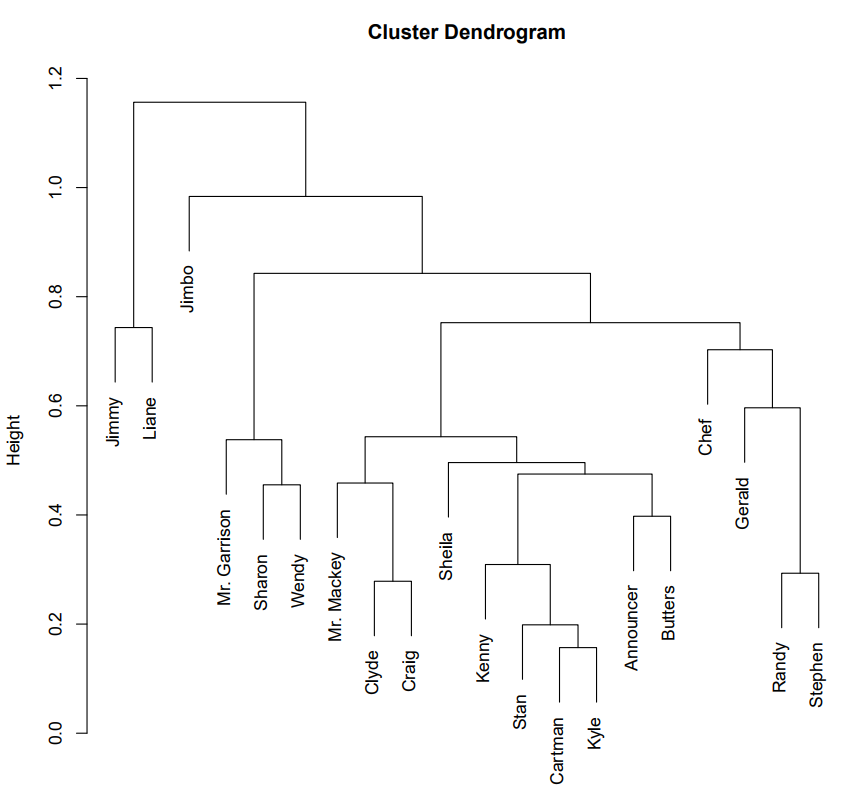
\includegraphics[scale=0.4]{images/Dendrogram.png}
	\caption{Cluster dendrogram of 20 major South Park characters}
	\label{fig:Dendrogram}
	\end{figure}
	\FloatBarrier
	\newpage
	\subsection{Sentiment and Emotion Mining}
	Another approach to learn something about South Park is to extract the sentiments and emotions that are expressed by the characters. The sentiments are annotated onto the seasons, using the Annotator provided by the \textbf{NLP} packag.
	
	After the complete corpus has been annotated, which results in little chunks of words being tied together, the sentiments are processed with the library \textbf{syuzhet} and the sentiment dictionary \textit{nrc}.
	During the processing the word chunks are grouped with 100 chunks being aggregated. Under the assumption that each character line contains at least 1 chunk, this results in a minimum of 700 grouped chunks for 70000 character lines, which can be seen as roughly three different sentiment values for each episode. This can be visualized with a sentiment timeline, as can be seen in Figures~\ref{fig:sentimentInitAll} and~\ref{fig:sentimentInit18}. One interesting observation is that the sentiments in Figure~\ref{fig:sentimentInit18} for season 18 are mostly positive with only a few segments having a negative sentiment score.
		
	\begin{figure}[!h]
  \centering
  \begin{minipage}[b]{0.45\textwidth}
    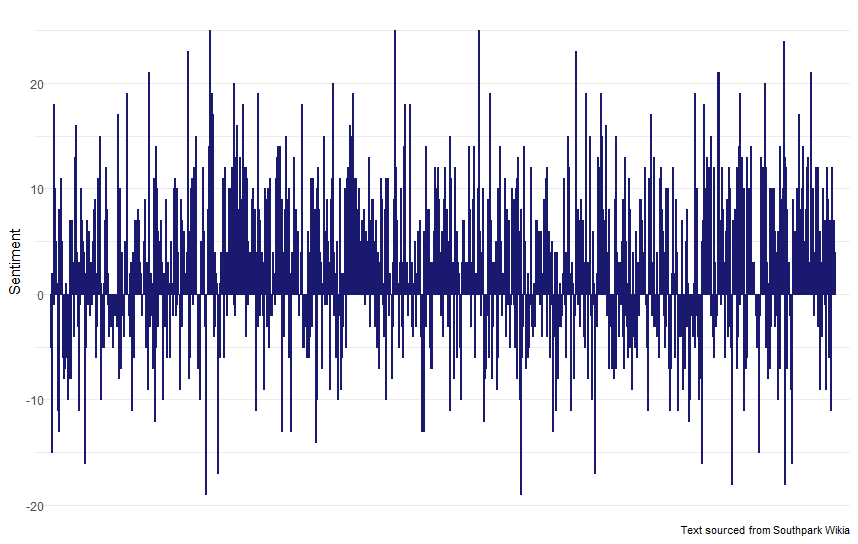
\includegraphics[width=\textwidth]{images/sentimentInitAll.png}
    \caption{Sentiment timeline over 18 seasons}
	\label{fig:sentimentInitAll}
  \end{minipage}
  \hfill
  \begin{minipage}[b]{0.45\textwidth}
    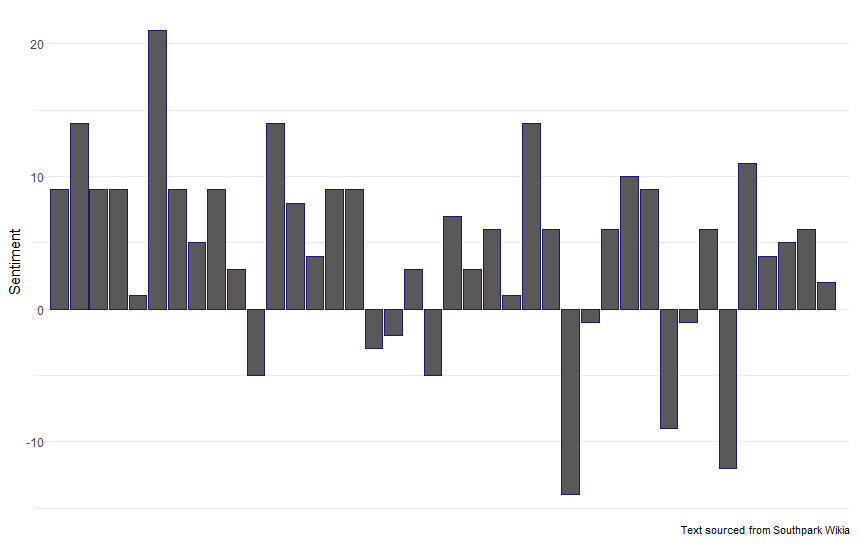
\includegraphics[width=\textwidth]{images/sentimentInit18.png}
    \caption{Sentiment timeline for season 18}
	\label{fig:sentimentInit18}
  \end{minipage}
\end{figure}

However, it is hard to derive a meaning from the sentiments that are shown in Figure~\ref{fig:sentimentInitAll}. Therefore, I decided to filter and transform the sentiment timelines with a low-pass Fourier transform using a low-pass size of 3. The Fourier Transform puts the data into a periodic shape, as can be seen in Figures~\ref{fig:sentimentFourierAll} and~\ref{fig:sentimentFourier18}.
		
	
	
	\begin{figure}[!h]
  \centering
  \begin{minipage}[b]{0.45\textwidth}
    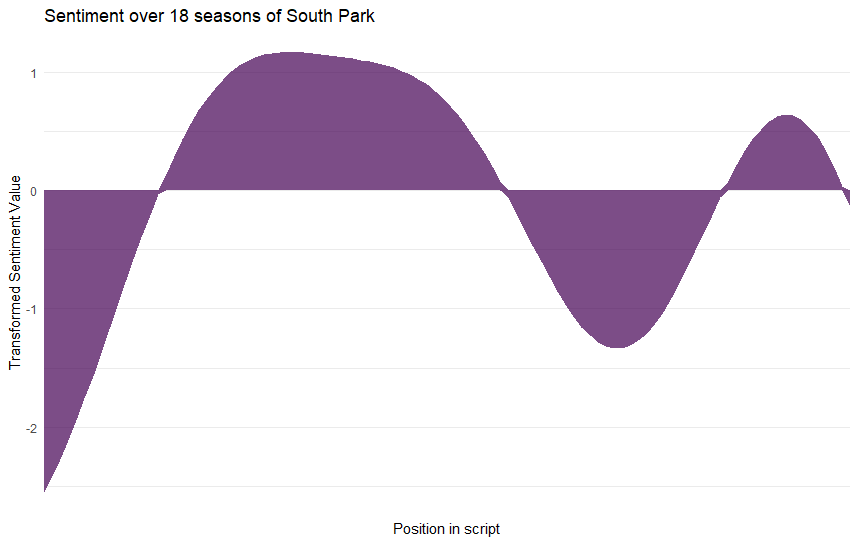
\includegraphics[width=\textwidth]{images/sentimentAll.png}
    \caption{Fourier transformed sentiment timeline over 18 seasons}
	\label{fig:sentimentFourierAll}
  \end{minipage}
  \hfill
  \begin{minipage}[b]{0.45\textwidth}
    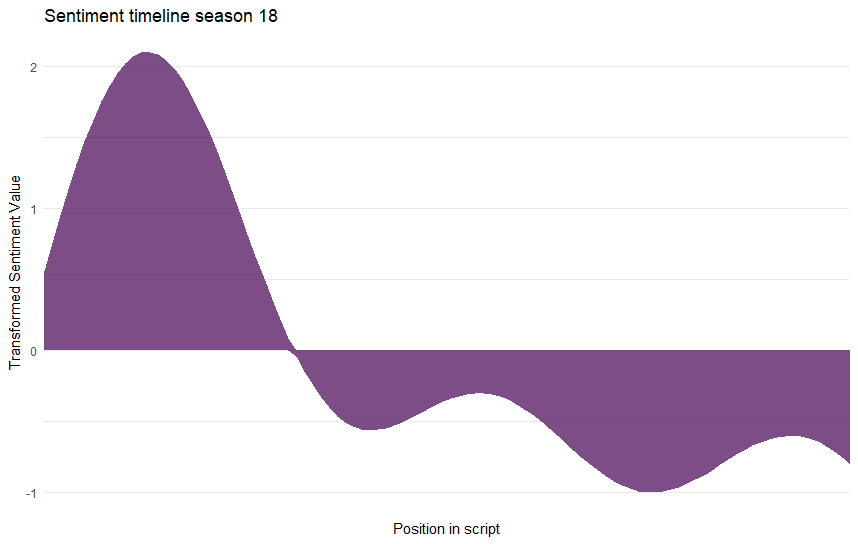
\includegraphics[width=\textwidth]{images/sentiment18.png}
    \caption{Fourier transformed sentiment timeline for season 18}
	\label{fig:sentimentFourier18}
  \end{minipage}
\end{figure}		

	This shows that during the first few seasons, in relation to the rest of the show, the sentiments were mostly negative.
	
	To gain an insight into the emotions that are expressed in South Park, I aggregated all emotions that were extracted using the \textit{nrc} lexicon and visualize them in the bar charts in Figures~\ref{fig:EmotionAll} and~\ref{fig:Emotion18}. It can be derived that  the emotions are rather negative, with around 50\% more sadness than joy. Also, a lot of anger and fear are expressed throughout the show.
	
	
	\begin{figure}[!h]
  \centering
  \begin{minipage}[b]{0.45\textwidth}
    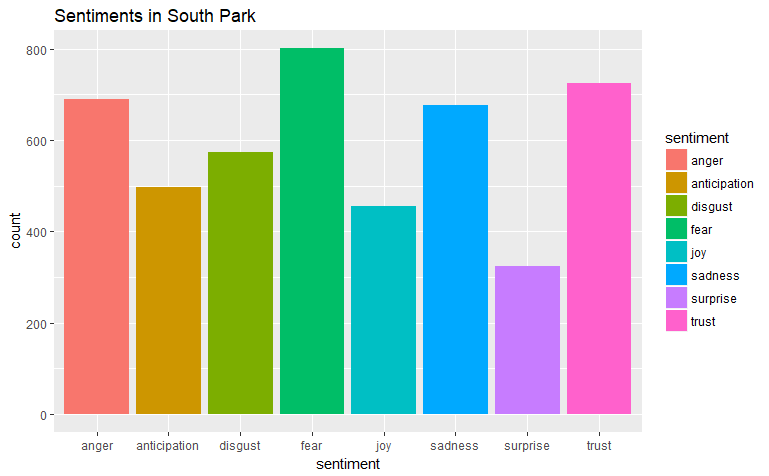
\includegraphics[width=\textwidth]{images/SentimentsSouthPark.png}
    \caption{Emotions over 18 seasons}
	\label{fig:EmotionAll}
  \end{minipage}
  \hfill
  \begin{minipage}[b]{0.45\textwidth}
    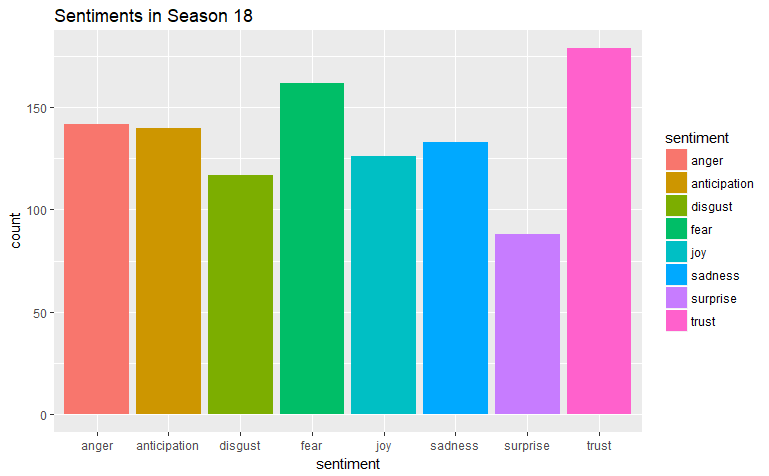
\includegraphics[width=\textwidth]{images/SentimentsSeason18.png}
    \caption{Emotions for season 18}
	\label{fig:Emotion18}
  \end{minipage}
\end{figure}		
	
				
	\FloatBarrier
	\subsection{Non-negative Matrix Factorization}
	The Non-negative Matrix Factorization (NMF) introduces the possibility to cluster documents in a TermDocumentMatrix by topic. For this implementation, the \textit{by.season} corpus was used, which after pre-processing was turned into a TDM with a maximum sparsity of 40\% allowed. The execution of the NMF algorithm provided by package \textbf{nmf} results in the coefficient and basis matrices. The coefficient map in Figure~\ref{fig:nmf} shows the clusters that are calculated for the seasons. The corresponding basis map that shows the most important words for each cluster is appended to the report\footnote{\textit{NMF\_basemap.pdf}}.
	
	
	\begin{figure}[h]
	\centering
	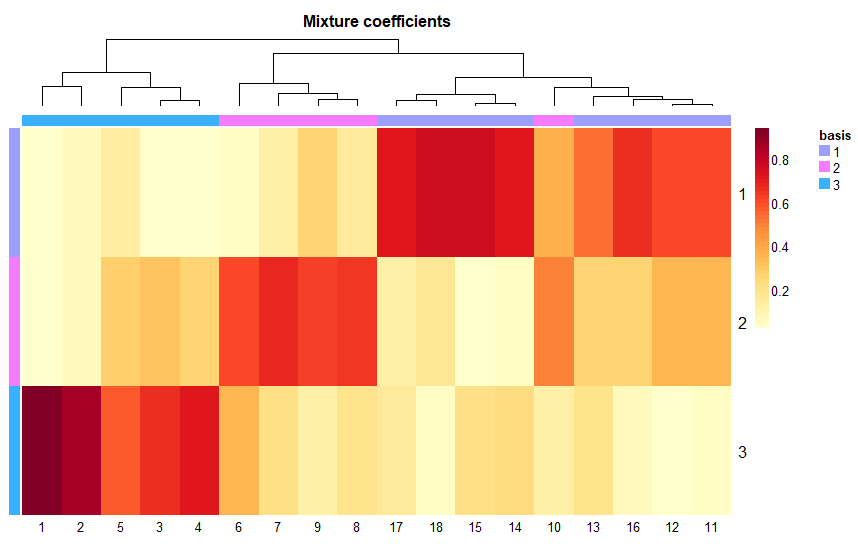
\includegraphics[scale=0.5]{images/NMF_coefmap.png}
	\caption{NMF topic clusters}
	\label{fig:nmf}
	\end{figure}
	
	The seasons are clustered with seasons 1-5, 6-9 and 10-18 being grouped together. To try to understand why they are clustered like this, I looked into the IMDb page\footnote{\url{http://www.imdb.com/title/tt0121955/}} of South Park and was able to find interesting correspondences, with major changes in writing in years 2001 and 2002(Figure~\ref{fig:nmfWriters}) and producing in 2006(Figure~\ref{fig:nmfProd}).
	
		\begin{figure}[!h]
  \centering
  \begin{minipage}[b]{0.45\textwidth}
   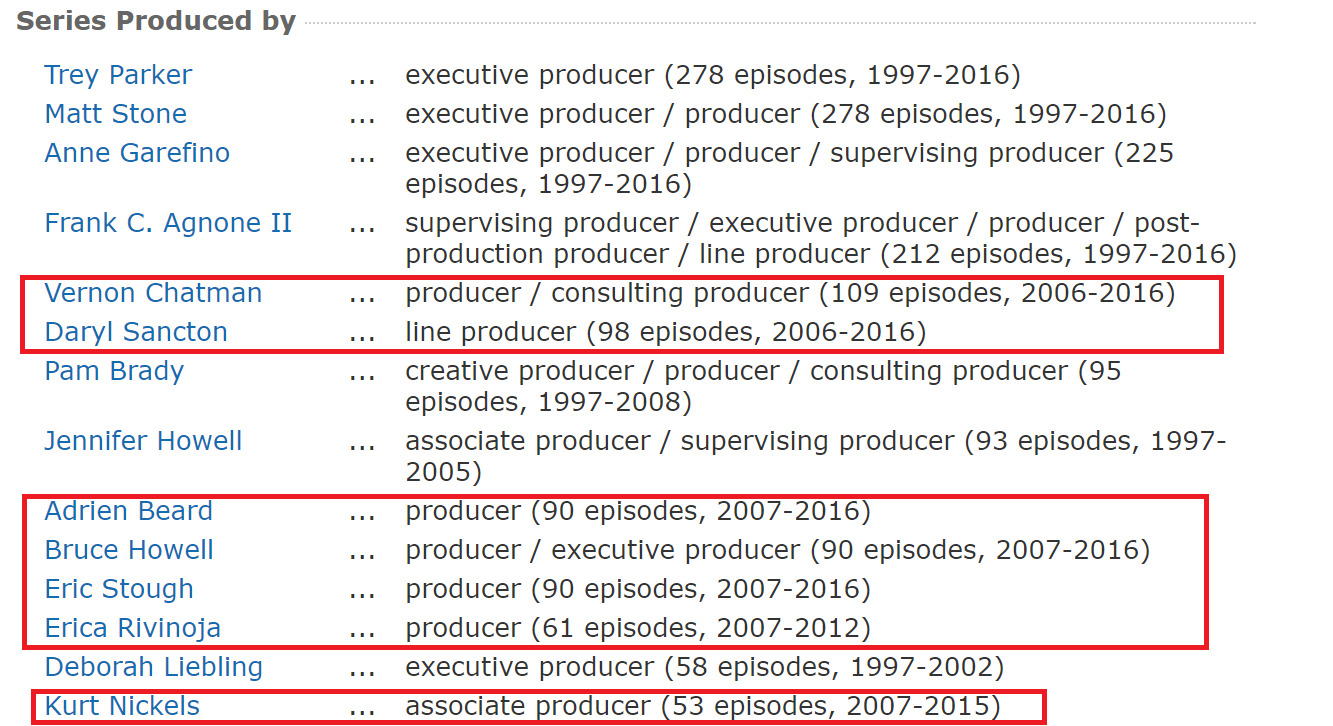
\includegraphics[width=\textwidth]{images/producer.png}
	\caption{Changes in producing}
	\label{fig:nmfProd}
  \end{minipage}
  \hfill
  \begin{minipage}[b]{0.45\textwidth}
   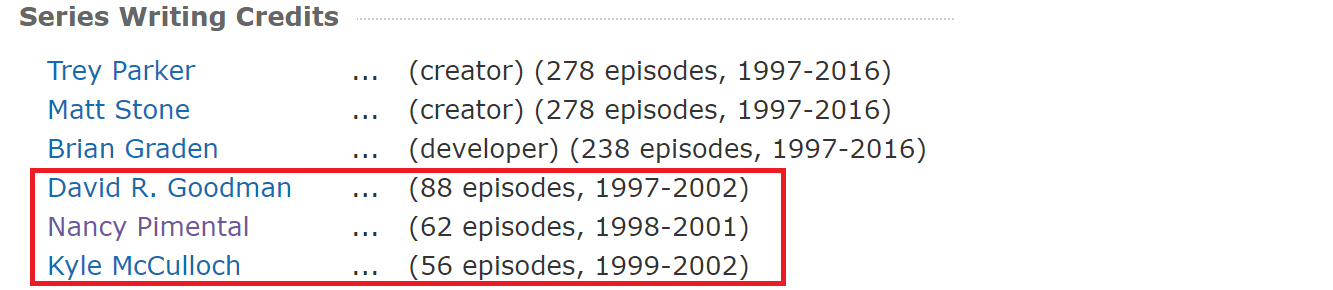
\includegraphics[width=\textwidth]{images/writers.png}
	\caption{Changes in writing}
	\label{fig:nmfWriters}
  \end{minipage}
\end{figure}		
	
	

	This corresponds to the different clusters obtained by the NMF, with Season 6 airing in 2002 and Season 10 airing in 2006, so it can be argued that the clusters are related to changes in the overall production of the show, namely writing and producing.
	
	\FloatBarrier
	\newpage
	\subsection{Structural Topic Model}
	Because the visualization of the basis map of the NMF doesn't provide an interactive way to inspect the topics and look at their most frequent terms, and to gain further insights into the topics that define South Park, I decided to use the \textbf{stm} package which provides the Structural Topic Model. Basically, \textbf{stm} is similar to other probabilistic topic models like the Latent Dirichlet Allocation(LDA). However, it allows to incorporate metadata into the topic model and enables the user to discover the main topics in a text corpus with a connection to the metadata. 
	
	To model the topics for all 18 seasons and season 18 only, the \textit{by.episode} corpus is used and pre-processed using the \textit{textProcessor} provided by the \textbf{stm} package. 
	Afterwards, the processed corpora are prepared, removing frequent terms that appear in more than 25 documents for all seasons and in more than 4 documents for season 18 only.
	With the prepared corpora, the Structural Topic Model is executed, modeling 25 and 4 topics, respectively. Since South Park mostly covers different topics between episodes, there are a lot of possible topics. With limiting this to 25, the main topics of South Park can be extracted, as can be seen in Figure~\ref{fig:stmAll}.
	
	\begin{figure}[h]
	\centering
	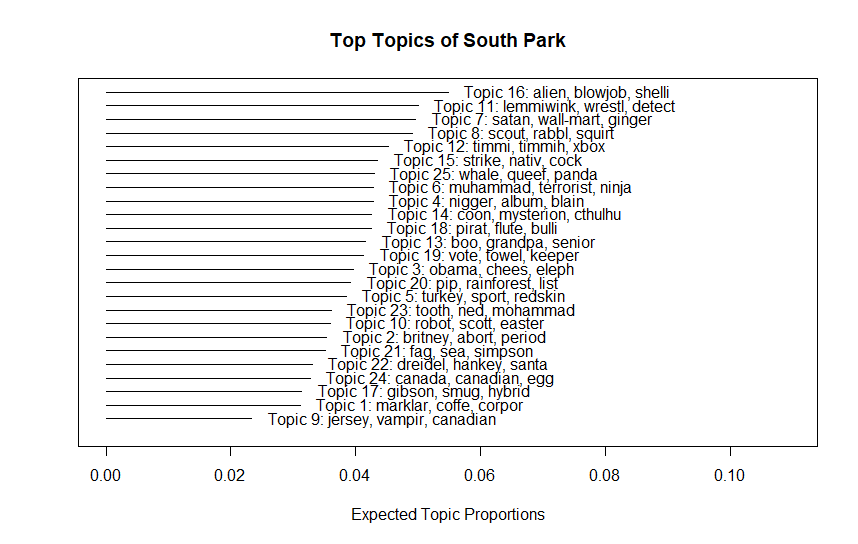
\includegraphics[scale=0.55]{images/TopicsAll.png}
	\caption{Structural Topic Model topics for South Park }
	\label{fig:stmAll}
	\end{figure}
	
	The most probable topic for each episode can be extracted and visualized. This can be seen in the topic timeline in Figure~\ref{fig:stmTimelineAll}. The results of this timeline seem to be accurate. As a sample to prove this, I chose topic 14 with the characteristic words "coon, mysterion, cthulhu" focusses on the superheroes saga around Coon, that appears in different seasons. In the topic timeline, there is a cluster shortly after episode 200 on the x-axis for topic 14. This relates to episodes 206 to, which is a 3 episode feature\footnote{E206 \textit{Coon 2: Hindsight}, E207 \textit{Mysterion Rises}, E208 \textit{Coon vs. Coon and Friends}} focussing on superheroes Coon and Mysterion.
	
	\begin{figure}[h]
	\centering
	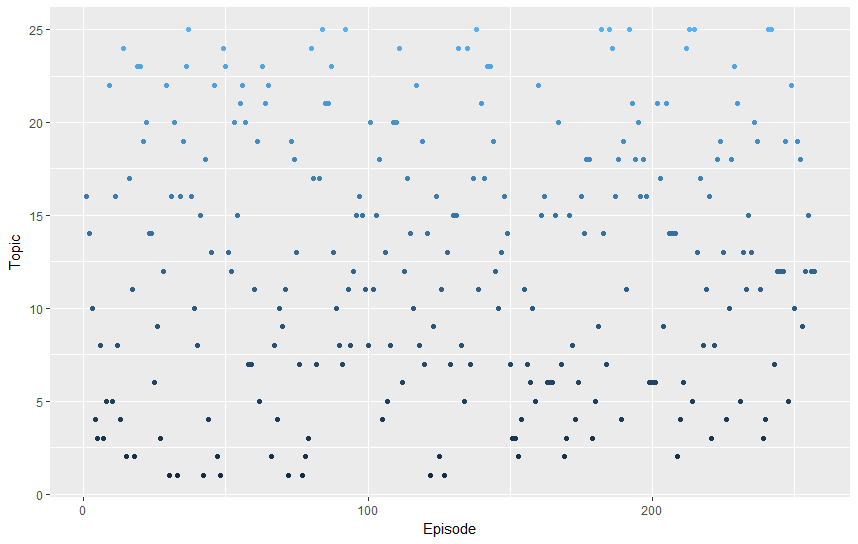
\includegraphics[scale=0.5]{images/TopicsAllTimeline.png}
	\caption{Topic timeline}
	\label{fig:stmTimelineAll}
	\end{figure}	
	
	To further inspect the different topics and gain insights into the clusters that have been calculated by the STM, I decided to use the package \textit{LDAvis} to visualize the different topics. Figure~\ref{fig:stmLDAvis} displays the generated topics.
	
	\begin{figure}[h]
	\centering
	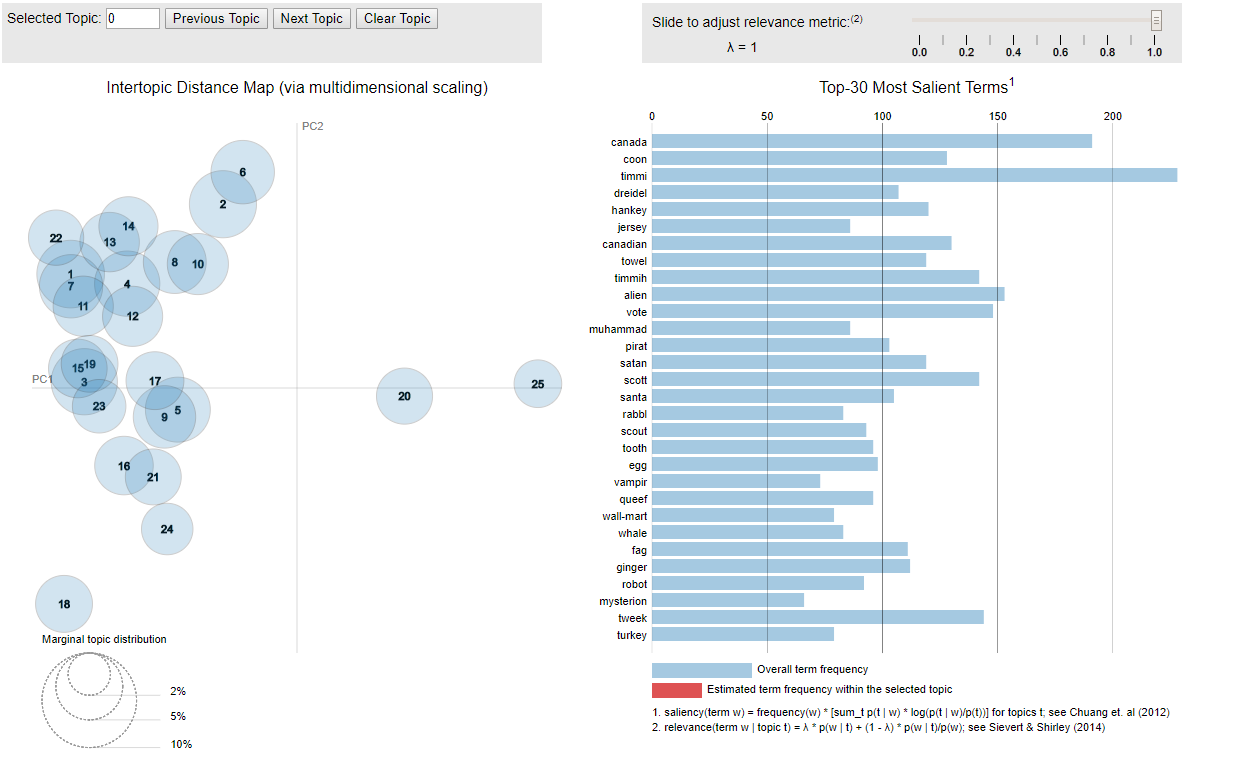
\includegraphics[scale=0.3]{images/LDAvis.png}
	\caption{STM visualization using LDAvis}
	\label{fig:stmLDAvis}
	\end{figure}	
	
	If the script \textit{stm.r} is executed, this will open the web browser, in which the topics can be inspected interactively, showing the estimated term frequency within the selected topic for the 30 most relevant terms per topic. Videos of this are appended to the report.
	
	All visualizations shown are appended to the report for only season 18 as well.\footnote{\textit{Topics18.png, Topics18Timeline}}
	
	\section{Conclusion}
	In conclusion, this report presented the different data sets that were used as well as the pre-processing that is applied to them in each case. Furthermore, the results and visualization were shown and a description as well as a reason for each result has been mentioned. The text mining of South Park has lead to a few observations, like the changes in writing and producing leading to different clusters of seasons or that the sentiment in the first few seasons of South Park were more negative than in later seasons.
	
	 To answer the combinations of W-questions, the topics extracted with the Structural Topic Model were visualized with a topic timeline that shows the most probable topic for each episode. This answers the combination of \textit{what-when}. 
	Also, a sentiment timeline for the show has been presented and discussed, answering the combination of \textit{why-when}.
	All images, scripts and data as well as videos displaying the Structural Topic Modeling are available in the GitHub repository.

	\section{Future work}
	To further increase the results, a few improvements could be introduced to the analysis of South Park.
	One possible future implementation is to visualize the sentiment and emotion timelines for different characters, which would then combine the three W-questions \textit{who, why}  and \textit{when}. This could lead to interesting results, with characters like Cartman being more aggressive than relaxed characters like Stan.
	Furthermore, the visualization of the topic timeline could be improved by creating a river plot that contains the content of the topics.
\end{document}
